% !TeX spellcheck = cs_CZ
\begin{example}Výstřel z děla (ve vakuu).
  Dělová koule opouští hlaveň zadanou rychlostí. Určete:
  \begin{itemize}\addtolength{\itemsep}{-0.5\baselineskip}
    \item maximální dostřel pro zadanou úsťovou rychlost,
    \item hranice oblasti, ve kterém lze zasáhnout cíl,
    \item stanovte velikost potřebného náměru děla pro zasažení libovolného cíle uvnitř ochranné paraboly.
  \end{itemize}

  {\centering
  \begin{tabular}{c}
       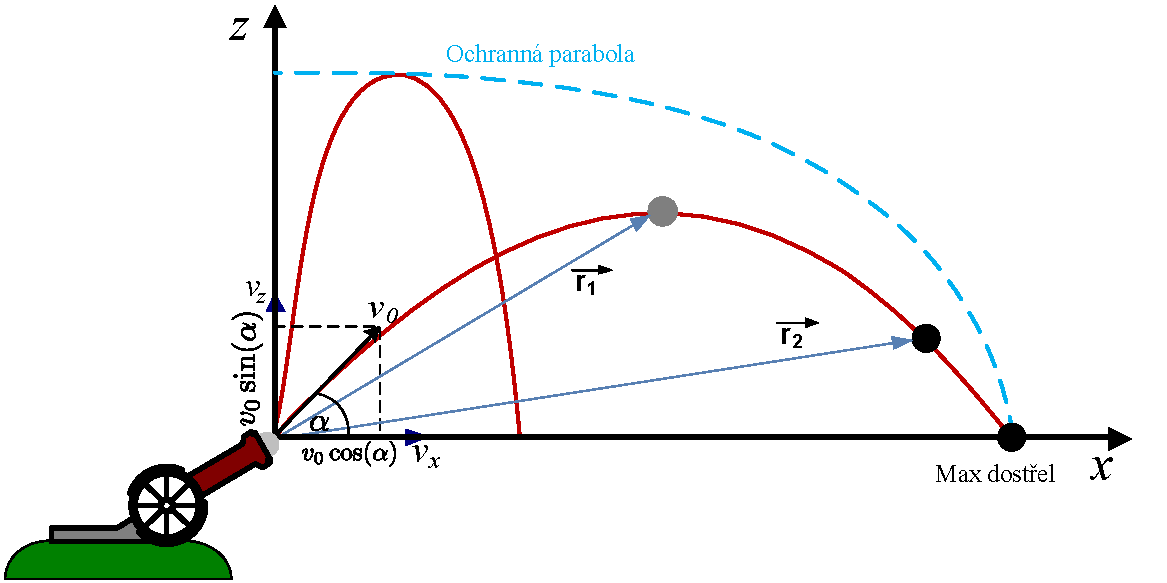
\includegraphics[width=0.9\linewidth]{fyz_fig223a.pdf}      \\
       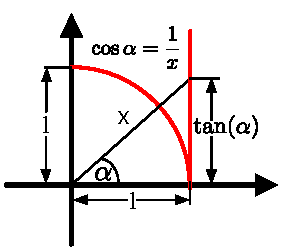
\includegraphics[width=0.3\linewidth]{fyz_fig223b.pdf}
  \end{tabular} 
  \captionsetup{type=figure}  
  \captionof{figure}{K příkladu výpočtu trajektorie projektilu. Goniometrický vzorec
           $|\cos\alpha|=\frac{1}{\sqrt{1+\tan\alpha^2}}$ lze snadno odvodit z náčrtu
           pomocí Pythagorovy věty (Přepona pravoúhlého trojúhelníka je
           $\sqrt{1+\tan\alpha^2}$)}            
  \label{fyz:fig223}
  \par}

  \textbf{Řešení:}
  Uvažujme rovinný pohyb v rovině $xz$, přičemž v záporném směru osy $z$ má pohyb zrychlení 
  velikosti $g$. Ve směru osy $z$ tedy probíhá rovnoměrně zrychlený pohyb podle rov. 
  \ref{mech:eq_const_acc}. Vztáhneme-li počáteční podmínky k okamžiku \(t = 0\), máme
  \begin{equation}\label{mech_eq_delo_vakuum_osa_z}
    z(t)=z_0+v_{0z}t-\frac{1}{2}gt^2, \qquad v_z(t)=v_{0z}-gt
  \end{equation}
  Ve směru osy $x$ je pohyb rovnoměrný:
  \begin{equation}\label{mech_eq_delo_vakuum_osa_x}
    x(t)=x_0+v_{0x} t,\qquad v_x(t)=v_{0x}=\mathrm{konst}
  \end{equation}

  Dělová koule opouští hlaveň pod elevačním úhlem $\alpha$ za podmínek dle obr. 
  \ref{fyz:fig223} platí $x_0=0, z_0=0, v_{0x}=v_0\cos\alpha>0, v_{0z}=v_0\sin\alpha>0$. Jde 
  tedy o skládání \emph{rovnoměrného přímočarého pohybu s rychlostí} $v_0\cos\alpha$ ve směru osy 
  $x$ a svislého pohybu vzhůru. Získané rovnice
  \begin{equation}\label{mech:eq_delo_rce_pohybu}
    z(t)=v_{0z}t-\frac{1}{2}gt^2, \qquad x(t)=v_{0x}t
  \end{equation}
  představují \emph{parametrické rovnice trajektorie}. Vyloučíme-li z nich čas $t$, dostaneme 
  rovnici křivky v kartézských souřadnicích
  \begin{equation}\label{mech:eq_delo_vakuum_param_rce}
    z(x)=  \frac{v_{0z}}{v_{0x}}x-\frac{1}{2}\frac{g}{v_{0x}^2}x^2
        = x\tan\alpha-\frac{1}{2}\frac{g}{v_0^2\cos^2\alpha}x^2
  \end{equation}
  Nyní aplikujeme goniometrický vzorec
  \begin{equation*}
    |cos\alpha|=   \frac{1}{\sqrt{1+\tan^2\alpha}}\Rightarrow \frac{1}{\cos^2\alpha} 
               = 1+\tan^2\alpha
  \end{equation*}
  odvozený dle náčrtku na obrázku \ref{fyz:fig223} a dostáváme rovnici
  \begin{equation}\label{mech_eq_example_vysledna_rce}
    z(x)=x\tan\alpha-\frac{1}{2}\frac{g}{v_0^2}(1+\tan^2\alpha)x^2
  \end{equation}
  Pohyb projektilu (dělové koule) probíhá po stejné trajektorii, jako šikmý vrh v homogenním 
  tíhovém poli ve vakuu, tedy po parabole. Snadno dostaneme \emph{souřadnice vrcholu dráhy, dálku 
  doletu a celkovou dobu letu}.

  \begin{itemize}
    \item Maximální dolet pro daný elevační úhel:
      \begin{equation}\label{mech:eq_elevacni_uhel_1}
        0=x\tan\alpha-\frac{1}{2}\frac{g}{v_0^2}(1+\tan^2\alpha)x^2
      \end{equation}
      \emph{Netriviální kořen této kvadratické rovnice je námi hledaný dolet dělové koule}
      \begin{align}  %\label{FYZ:eq235}
        x_d &=\frac{2v_0^2\tan\alpha}{g(1+\tan^2\alpha)}(1+\tan^2\alpha)        \nonumber \\
            &=\frac{2v_0^2\sin\alpha\cos\alpha}{g}=\frac{v_0^2\sin{2\alpha}}{g} \label{FYZ:eq235}
      \end{align}

    \item Celková doba letu:
      \begin{equation}\label{mech:eq_doba_letu}
        t_d=\frac{x_d}{v_{0x}} =\frac{2v_0^2\sin\alpha\cos\alpha}{gv_0\cos\alpha}
           =\frac{2v_0\sin\alpha}{g}
      \end{equation}

    \item Souřadnice vrcholu dráhy: \emph{získáme derivováním rov.
          \ref{mech_eq_example_vysledna_rce}}
          \begin{align}
            0   &= tan\alpha-\frac{g}{v_0^2(1+\tan^2\alpha)}x_v                         \\
            x_v &= \frac{v_0^2}{g}\frac{\tan\alpha}{1+\tan^2\alpha}=
                   \frac{v_0^2}{g}\frac{\sin\alpha}{\cos\alpha}
                   \cdot\cos^2\alpha\cdot\frac{2}{2}                                   \\
            x_v &= \frac{v_0^2\sin{2\alpha}}{2g}
           \end{align}
           \emph{Souřadnici $z_v$ dostaneme dosazením $x_v$  do rov.
           \ref{mech_eq_example_vysledna_rce}}
           \begin{align*}
             z_v &= \frac{v_0^2}{g}\frac{\tan^2\alpha}{1+\tan^2\alpha}-
                    \frac{1}{2}\frac{g}{v_0^2}(1+\tan^2\alpha)\frac{v_0^4}{g^2}
                    \frac{\tan^2\alpha}{(1+\tan^2\alpha)^2}                            \\
             z_v &= \frac{v_0^2}{g}\frac{\tan^2\alpha}{1+\tan^2\alpha}-
                    \frac{1}{2}\frac{v_0^2}{g}\frac{\tan^2\alpha}{1+\tan^2\alpha}      \\
             z_v &= \frac{v_0^2\sin^2\alpha}{2g}
      \end{align*}
      \emph{Odtud je zřejmé, že maximální délka doletu odpovídá úhlu $\frac{\pi}{4}$ a že obecně 
      daného bodu doletu lze dosáhnout pod dvěma různými úhly $\frac{\pi}{4}\pm\Delta\alpha$.}

    \item Stanovení elevačního úhlu pro zasažení zadaných souřadnic $[X_c, Z_c]$ cíle: \emph{Opět  
          vycházíme z rov. \ref{mech_eq_example_vysledna_rce}, ovšem tentokrát nejsou neznáme $x$ a 
          $z$, ale $\alpha$: Použijeme substituci $\tan\alpha=p$ a vypočítáme kořeny této 
          kvadratické rovnice:}
          \begin{align}
            0       &= gx^2p^2-2v_0^2xp+(gx^2+2zv_0^2) \\
            p_{1,2} &= \frac{v_0^2\pm\sqrt{v_0^4-g(gx^2+2zv_0^2)}}{gx} \\
            \alpha  &= \tan^{-1}\left(\frac{v_0^2\pm\sqrt{v_0^4-g(gx^2+2zv_0^2)}}{gx}\right)
          \end{align}
          \emph{Je-li cíl zadán v polárních souřadnicích $[r,\varphi]$, lze potřebný náměr stanovit takto:}
          \begin{equation*}
            \alpha=\tan^{-1}\left(\frac{v_0^2\pm
                   \sqrt{v_0^4-g(gr^2\cos^2\varphi+2r\sin\varphi
                         v_0^2)}}{gr\cos\varphi}\right)
          \end{equation*}
          \emph{Pokud ovšem bude diskriminant menší než 0, leží cíl mimo dosah děla. Tj. neexistuje 
          takový náměr děla, kterým by bylo možné cíl zasáhnout. Je-li diskriminant roven nule, 
          jedná se o hranici, za kterou již při dané úsťové rychlosti nelze dostřelit. Body ležící 
          na této obálce tzv. ochranná parabola mohou být zasaženy pouze při jedné hodnotě 
          elevačního úhlu.}

    \item Stanovení rovnice ochranné paraboly: \emph{To provedeme tak, že položíme diskriminant 	
          rovnice pro $\tan\alpha$ roven nule a dostaneme rovnici obálky}
          \begin{equation}\label{mech:eq_ochr_parabola}
            v_0^4-g(gx^2+2zv_0^2)\Rightarrow z=-\frac{v_0^2}{2g^2}x^2+\frac{v_0^2}{2g}
          \end{equation}
  \end{itemize}

  %------------------------------Dělo---------------------------------
  \lstinputlisting{../src/FYZ/matlab/kinematika_delo_ve_vakuu.m}
  \begin{lstlisting}[caption=\texttt{kinematika\_delo\_ve\_vakuu.m} pro ověření výpočtu 
  balistické dráhy projektilu.]
  \end{lstlisting}
  %-------------------------------------------------------------------
  {\centering
    \captionsetup{type=figure}
   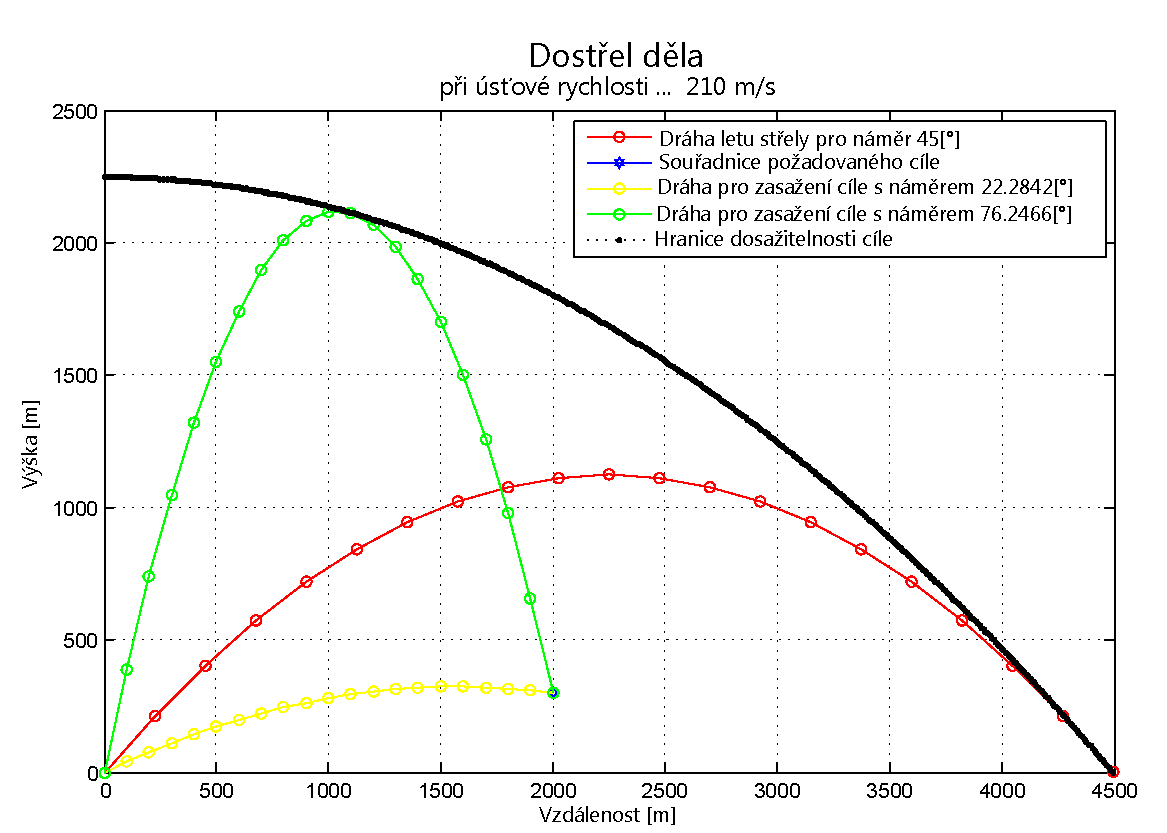
\includegraphics[width=\linewidth]{fyz_fig222.pdf}
    \captionof{figure}{Výpočet trajektorie projektilu ve vakuu při úsťové rychlosti $210 m/s$ 
              pomocí sw MATLAB\textsuperscript{\textregistered}.}
    \label{mech:fig_delo_matlab}
  \par}
\end{example}